\documentclass[twoside]{book}

% Packages required by doxygen
\usepackage{fixltx2e}
\usepackage{calc}
\usepackage{doxygen}
\usepackage[export]{adjustbox} % also loads graphicx
\usepackage{graphicx}
\usepackage[utf8]{inputenc}
\usepackage{makeidx}
\usepackage{multicol}
\usepackage{multirow}
\PassOptionsToPackage{warn}{textcomp}
\usepackage{textcomp}
\usepackage[nointegrals]{wasysym}
\usepackage[table]{xcolor}

% Font selection
\usepackage[T1]{fontenc}
\usepackage[scaled=.90]{helvet}
\usepackage{courier}
\usepackage{amssymb}
\usepackage{sectsty}
\renewcommand{\familydefault}{\sfdefault}
\allsectionsfont{%
  \fontseries{bc}\selectfont%
  \color{darkgray}%
}
\renewcommand{\DoxyLabelFont}{%
  \fontseries{bc}\selectfont%
  \color{darkgray}%
}
\newcommand{\+}{\discretionary{\mbox{\scriptsize$\hookleftarrow$}}{}{}}

% Page & text layout
\usepackage{geometry}
\geometry{%
  a4paper,%
  top=2.5cm,%
  bottom=2.5cm,%
  left=2.5cm,%
  right=2.5cm%
}
\tolerance=750
\hfuzz=15pt
\hbadness=750
\setlength{\emergencystretch}{15pt}
\setlength{\parindent}{0cm}
\setlength{\parskip}{3ex plus 2ex minus 2ex}
\makeatletter
\renewcommand{\paragraph}{%
  \@startsection{paragraph}{4}{0ex}{-1.0ex}{1.0ex}{%
    \normalfont\normalsize\bfseries\SS@parafont%
  }%
}
\renewcommand{\subparagraph}{%
  \@startsection{subparagraph}{5}{0ex}{-1.0ex}{1.0ex}{%
    \normalfont\normalsize\bfseries\SS@subparafont%
  }%
}
\makeatother

% Headers & footers
\usepackage{fancyhdr}
\pagestyle{fancyplain}
\fancyhead[LE]{\fancyplain{}{\bfseries\thepage}}
\fancyhead[CE]{\fancyplain{}{}}
\fancyhead[RE]{\fancyplain{}{\bfseries\leftmark}}
\fancyhead[LO]{\fancyplain{}{\bfseries\rightmark}}
\fancyhead[CO]{\fancyplain{}{}}
\fancyhead[RO]{\fancyplain{}{\bfseries\thepage}}
\fancyfoot[LE]{\fancyplain{}{}}
\fancyfoot[CE]{\fancyplain{}{}}
\fancyfoot[RE]{\fancyplain{}{\bfseries\scriptsize Generated by Doxygen }}
\fancyfoot[LO]{\fancyplain{}{\bfseries\scriptsize Generated by Doxygen }}
\fancyfoot[CO]{\fancyplain{}{}}
\fancyfoot[RO]{\fancyplain{}{}}
\renewcommand{\footrulewidth}{0.4pt}
\renewcommand{\chaptermark}[1]{%
  \markboth{#1}{}%
}
\renewcommand{\sectionmark}[1]{%
  \markright{\thesection\ #1}%
}

% Indices & bibliography
\usepackage{natbib}
\usepackage[titles]{tocloft}
\setcounter{tocdepth}{3}
\setcounter{secnumdepth}{5}
\makeindex

% Hyperlinks (required, but should be loaded last)
\usepackage{ifpdf}
\ifpdf
  \usepackage[pdftex,pagebackref=true]{hyperref}
\else
  \usepackage[ps2pdf,pagebackref=true]{hyperref}
\fi
\hypersetup{%
  colorlinks=true,%
  linkcolor=blue,%
  citecolor=blue,%
  unicode%
}

% Custom commands
\newcommand{\clearemptydoublepage}{%
  \newpage{\pagestyle{empty}\cleardoublepage}%
}

\usepackage{caption}
\captionsetup{labelsep=space,justification=centering,font={bf},singlelinecheck=off,skip=4pt,position=top}

%===== C O N T E N T S =====

\begin{document}

% Titlepage & ToC
\hypersetup{pageanchor=false,
             bookmarksnumbered=true,
             pdfencoding=unicode
            }
\pagenumbering{alph}
\begin{titlepage}
\vspace*{7cm}
\begin{center}%
{\Large My Project }\\
\vspace*{1cm}
{\large Generated by Doxygen 1.8.13}\\
\end{center}
\end{titlepage}
\clearemptydoublepage
\pagenumbering{roman}
\tableofcontents
\clearemptydoublepage
\pagenumbering{arabic}
\hypersetup{pageanchor=true}

%--- Begin generated contents ---
\chapter{Hierarchical Index}
\section{类继承关系}
此继承关系列表按字典顺序粗略的排序\+: \begin{DoxyCompactList}
\item N\+S\+Object\begin{DoxyCompactList}
\item \contentsline{section}{Offline\+Play\+Back}{\pageref{interface_offline_play_back}}{}
\item \contentsline{section}{Play\+Parameter}{\pageref{interface_play_parameter}}{}
\item \contentsline{section}{Request\+Data}{\pageref{interface_request_data}}{}
\item \contentsline{section}{Request\+Data\+Play\+Back}{\pageref{interface_request_data_play_back}}{}
\item \contentsline{section}{Save\+Log\+Util}{\pageref{interface_save_log_util}}{}
\end{DoxyCompactList}
\item $<$N\+S\+Object$>$\begin{DoxyCompactList}
\item \contentsline{section}{$<$Offline\+Play\+Back\+Delegate $>$}{\pageref{protocol_offline_play_back_delegate_01-p}}{}
\item \contentsline{section}{$<$Request\+Data\+Delegate $>$}{\pageref{protocol_request_data_delegate_01-p}}{}
\item \contentsline{section}{$<$Request\+Data\+Play\+Back\+Delegate $>$}{\pageref{protocol_request_data_play_back_delegate_01-p}}{}
\end{DoxyCompactList}
\end{DoxyCompactList}

\chapter{Class Index}
\section{类列表}
这里列出了所有类、结构、联合以及接口定义等,并附带简要说明\+:\begin{DoxyCompactList}
\item\contentsline{section}{\hyperlink{interface_offline_play_back}{Offline\+Play\+Back} }{\pageref{interface_offline_play_back}}{}
\item\contentsline{section}{\hyperlink{protocol_offline_play_back_delegate_01-p}{$<$\+Offline\+Play\+Back\+Delegate $>$} }{\pageref{protocol_offline_play_back_delegate_01-p}}{}
\item\contentsline{section}{\hyperlink{interface_play_parameter}{Play\+Parameter} }{\pageref{interface_play_parameter}}{}
\item\contentsline{section}{\hyperlink{interface_request_data}{Request\+Data} }{\pageref{interface_request_data}}{}
\item\contentsline{section}{\hyperlink{protocol_request_data_delegate_01-p}{$<$\+Request\+Data\+Delegate $>$} }{\pageref{protocol_request_data_delegate_01-p}}{}
\item\contentsline{section}{\hyperlink{interface_request_data_play_back}{Request\+Data\+Play\+Back} }{\pageref{interface_request_data_play_back}}{}
\item\contentsline{section}{\hyperlink{protocol_request_data_play_back_delegate_01-p}{$<$\+Request\+Data\+Play\+Back\+Delegate $>$} }{\pageref{protocol_request_data_play_back_delegate_01-p}}{}
\item\contentsline{section}{\hyperlink{interface_save_log_util}{Save\+Log\+Util} }{\pageref{interface_save_log_util}}{}
\end{DoxyCompactList}

\chapter{Class Documentation}
\hypertarget{interface_i_j_k_a_v_movie_player_controller}{}\section{I\+J\+K\+A\+V\+Movie\+Player\+Controller Class Reference}
\label{interface_i_j_k_a_v_movie_player_controller}\index{I\+J\+K\+A\+V\+Movie\+Player\+Controller@{I\+J\+K\+A\+V\+Movie\+Player\+Controller}}
Inheritance diagram for I\+J\+K\+A\+V\+Movie\+Player\+Controller\+:\begin{figure}[H]
\begin{center}
\leavevmode
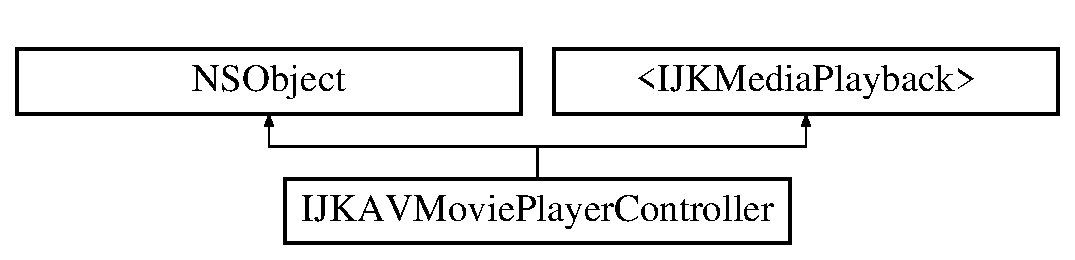
\includegraphics[height=2.000000cm]{interface_i_j_k_a_v_movie_player_controller}
\end{center}
\end{figure}
\subsection*{Instance Methods}
\begin{DoxyCompactItemize}
\item 
\mbox{\Hypertarget{interface_i_j_k_a_v_movie_player_controller_aa5577992e0ec0e08d005551db18a7404}\label{interface_i_j_k_a_v_movie_player_controller_aa5577992e0ec0e08d005551db18a7404}} 
(id) -\/ {\bfseries init\+With\+Content\+U\+R\+L\+:}
\item 
\mbox{\Hypertarget{interface_i_j_k_a_v_movie_player_controller_aab57326b5b5d69b8ef1b16d1da2d0c59}\label{interface_i_j_k_a_v_movie_player_controller_aab57326b5b5d69b8ef1b16d1da2d0c59}} 
(id) -\/ {\bfseries init\+With\+Content\+U\+R\+L\+String\+:}
\end{DoxyCompactItemize}
\subsection*{Class Methods}
\begin{DoxyCompactItemize}
\item 
\mbox{\Hypertarget{interface_i_j_k_a_v_movie_player_controller_aba8ce410fac68355c28f134003f9d7eb}\label{interface_i_j_k_a_v_movie_player_controller_aba8ce410fac68355c28f134003f9d7eb}} 
(id) + {\bfseries get\+Instance\+:}
\end{DoxyCompactItemize}


The documentation for this class was generated from the following file\+:\begin{DoxyCompactItemize}
\item 
I\+J\+K\+A\+V\+Movie\+Player\+Controller.\+h\end{DoxyCompactItemize}

\hypertarget{interface_i_j_k_f_f_monitor}{}\section{I\+J\+K\+F\+F\+Monitor Class Reference}
\label{interface_i_j_k_f_f_monitor}\index{I\+J\+K\+F\+F\+Monitor@{I\+J\+K\+F\+F\+Monitor}}
Inheritance diagram for I\+J\+K\+F\+F\+Monitor\+:\begin{figure}[H]
\begin{center}
\leavevmode
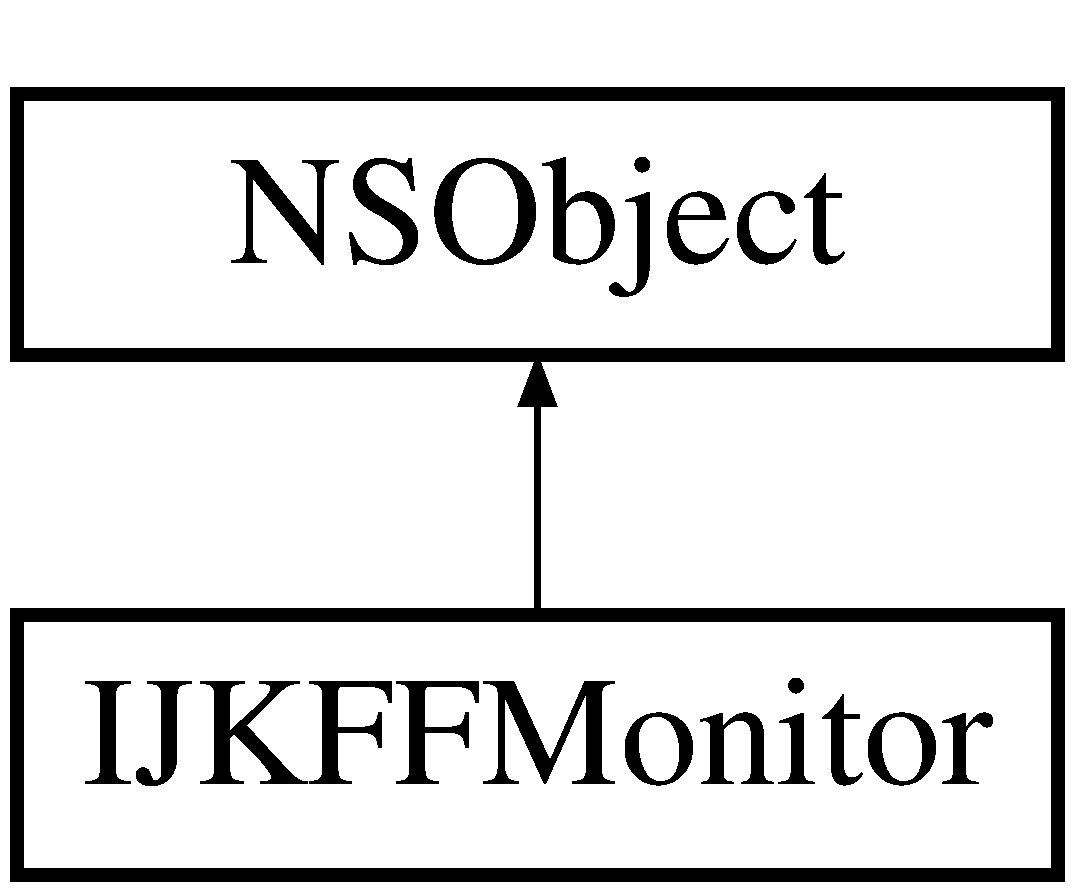
\includegraphics[height=2.000000cm]{interface_i_j_k_f_f_monitor}
\end{center}
\end{figure}
\subsection*{Instance Methods}
\begin{DoxyCompactItemize}
\item 
\mbox{\Hypertarget{interface_i_j_k_f_f_monitor_adfe6ec9e9decc829bfcd501f38366f18}\label{interface_i_j_k_f_f_monitor_adfe6ec9e9decc829bfcd501f38366f18}} 
(instancetype) -\/ {\bfseries init}
\end{DoxyCompactItemize}
\subsection*{Properties}
\begin{DoxyCompactItemize}
\item 
\mbox{\Hypertarget{interface_i_j_k_f_f_monitor_ab4bde5f27d12c0fa7e0c45dc3e0865aa}\label{interface_i_j_k_f_f_monitor_ab4bde5f27d12c0fa7e0c45dc3e0865aa}} 
N\+S\+Dictionary $\ast$ {\bfseries media\+Meta}
\item 
\mbox{\Hypertarget{interface_i_j_k_f_f_monitor_a77f9c2492e9c77025d9dc1d713a209c1}\label{interface_i_j_k_f_f_monitor_a77f9c2492e9c77025d9dc1d713a209c1}} 
N\+S\+Dictionary $\ast$ {\bfseries video\+Meta}
\item 
\mbox{\Hypertarget{interface_i_j_k_f_f_monitor_ad093c561eab0e108eb90ea48dbd97b89}\label{interface_i_j_k_f_f_monitor_ad093c561eab0e108eb90ea48dbd97b89}} 
N\+S\+Dictionary $\ast$ {\bfseries audio\+Meta}
\item 
\mbox{\Hypertarget{interface_i_j_k_f_f_monitor_af54130281bae20143bff32943fa3365a}\label{interface_i_j_k_f_f_monitor_af54130281bae20143bff32943fa3365a}} 
int64\+\_\+t {\bfseries duration}
\item 
\mbox{\Hypertarget{interface_i_j_k_f_f_monitor_a4073f3b5100932679a91ead73bcd77c4}\label{interface_i_j_k_f_f_monitor_a4073f3b5100932679a91ead73bcd77c4}} 
int64\+\_\+t {\bfseries bitrate}
\item 
\mbox{\Hypertarget{interface_i_j_k_f_f_monitor_a8bfdb7d9c3fe856e619c1881a319659a}\label{interface_i_j_k_f_f_monitor_a8bfdb7d9c3fe856e619c1881a319659a}} 
float {\bfseries fps}
\item 
\mbox{\Hypertarget{interface_i_j_k_f_f_monitor_a866c2215f4ee63607d30dbf4d30b78e1}\label{interface_i_j_k_f_f_monitor_a866c2215f4ee63607d30dbf4d30b78e1}} 
int {\bfseries width}
\item 
\mbox{\Hypertarget{interface_i_j_k_f_f_monitor_a865f9ed0c9558559ba84cbacaa5f1046}\label{interface_i_j_k_f_f_monitor_a865f9ed0c9558559ba84cbacaa5f1046}} 
int {\bfseries height}
\item 
\mbox{\Hypertarget{interface_i_j_k_f_f_monitor_a25c995516fe73bedcdf43ba545540cad}\label{interface_i_j_k_f_f_monitor_a25c995516fe73bedcdf43ba545540cad}} 
N\+S\+String $\ast$ {\bfseries vcodec}
\item 
\mbox{\Hypertarget{interface_i_j_k_f_f_monitor_a03ff47710e58e11264e9228262d6b36c}\label{interface_i_j_k_f_f_monitor_a03ff47710e58e11264e9228262d6b36c}} 
N\+S\+String $\ast$ {\bfseries acodec}
\item 
\mbox{\Hypertarget{interface_i_j_k_f_f_monitor_a6167584e9834463cce724e3871ba9f8c}\label{interface_i_j_k_f_f_monitor_a6167584e9834463cce724e3871ba9f8c}} 
int {\bfseries sample\+Rate}
\item 
\mbox{\Hypertarget{interface_i_j_k_f_f_monitor_a749f490c30f3b8c47b0facc75f2ed293}\label{interface_i_j_k_f_f_monitor_a749f490c30f3b8c47b0facc75f2ed293}} 
int64\+\_\+t {\bfseries channel\+Layout}
\item 
\mbox{\Hypertarget{interface_i_j_k_f_f_monitor_acd8324d40f631d659d462a72a1b35a7b}\label{interface_i_j_k_f_f_monitor_acd8324d40f631d659d462a72a1b35a7b}} 
N\+S\+String $\ast$ {\bfseries vdecoder}
\item 
\mbox{\Hypertarget{interface_i_j_k_f_f_monitor_a2a81726e719824e11bc3398b3a4552ff}\label{interface_i_j_k_f_f_monitor_a2a81726e719824e11bc3398b3a4552ff}} 
int {\bfseries tcp\+Error}
\item 
\mbox{\Hypertarget{interface_i_j_k_f_f_monitor_a6034531c489463ee0ee49a8f8d55330d}\label{interface_i_j_k_f_f_monitor_a6034531c489463ee0ee49a8f8d55330d}} 
N\+S\+String $\ast$ {\bfseries remote\+Ip}
\item 
\mbox{\Hypertarget{interface_i_j_k_f_f_monitor_a73bd3ddd20e35b89b991f6cf8cf5a7bb}\label{interface_i_j_k_f_f_monitor_a73bd3ddd20e35b89b991f6cf8cf5a7bb}} 
int {\bfseries http\+Error}
\item 
\mbox{\Hypertarget{interface_i_j_k_f_f_monitor_aaf5e3623a9a6879d8a892fc608cbbe7d}\label{interface_i_j_k_f_f_monitor_aaf5e3623a9a6879d8a892fc608cbbe7d}} 
N\+S\+String $\ast$ {\bfseries http\+Url}
\item 
\mbox{\Hypertarget{interface_i_j_k_f_f_monitor_a52cfaf319058b73d5e0d2e4f504c1913}\label{interface_i_j_k_f_f_monitor_a52cfaf319058b73d5e0d2e4f504c1913}} 
N\+S\+String $\ast$ {\bfseries http\+Host}
\item 
\mbox{\Hypertarget{interface_i_j_k_f_f_monitor_a27c976704644ddc64f4a6ad38db4285b}\label{interface_i_j_k_f_f_monitor_a27c976704644ddc64f4a6ad38db4285b}} 
int {\bfseries http\+Code}
\item 
\mbox{\Hypertarget{interface_i_j_k_f_f_monitor_a201f6946cfd23b728824a0929d83eb7a}\label{interface_i_j_k_f_f_monitor_a201f6946cfd23b728824a0929d83eb7a}} 
int64\+\_\+t {\bfseries http\+Open\+Tick}
\item 
\mbox{\Hypertarget{interface_i_j_k_f_f_monitor_ada092094ce7a1b0d22e078892a529fcb}\label{interface_i_j_k_f_f_monitor_ada092094ce7a1b0d22e078892a529fcb}} 
int64\+\_\+t {\bfseries http\+Seek\+Tick}
\item 
\mbox{\Hypertarget{interface_i_j_k_f_f_monitor_ad8947b8f0ad5b7ac85dede0231b8a79a}\label{interface_i_j_k_f_f_monitor_ad8947b8f0ad5b7ac85dede0231b8a79a}} 
int {\bfseries http\+Open\+Count}
\item 
\mbox{\Hypertarget{interface_i_j_k_f_f_monitor_a58ad94d39e1ccd9cd576240f561e289d}\label{interface_i_j_k_f_f_monitor_a58ad94d39e1ccd9cd576240f561e289d}} 
int {\bfseries http\+Seek\+Count}
\item 
\mbox{\Hypertarget{interface_i_j_k_f_f_monitor_aa89a953d8a910128daa702b8cdf257ba}\label{interface_i_j_k_f_f_monitor_aa89a953d8a910128daa702b8cdf257ba}} 
int64\+\_\+t {\bfseries last\+Http\+Open\+Duration}
\item 
\mbox{\Hypertarget{interface_i_j_k_f_f_monitor_a14276356a7f783edf767b9982acee597}\label{interface_i_j_k_f_f_monitor_a14276356a7f783edf767b9982acee597}} 
int64\+\_\+t {\bfseries last\+Http\+Seek\+Duration}
\item 
\mbox{\Hypertarget{interface_i_j_k_f_f_monitor_a9f5930b8a180f604bf8bce0bf41102d7}\label{interface_i_j_k_f_f_monitor_a9f5930b8a180f604bf8bce0bf41102d7}} 
int64\+\_\+t {\bfseries prepare\+Start\+Tick}
\item 
\mbox{\Hypertarget{interface_i_j_k_f_f_monitor_ad33dfab180a43cdd0de4c1f50a8e4778}\label{interface_i_j_k_f_f_monitor_ad33dfab180a43cdd0de4c1f50a8e4778}} 
int64\+\_\+t {\bfseries prepare\+Duration}
\item 
\mbox{\Hypertarget{interface_i_j_k_f_f_monitor_a7c7db7e8f78b655b13253e730ab6c04b}\label{interface_i_j_k_f_f_monitor_a7c7db7e8f78b655b13253e730ab6c04b}} 
int64\+\_\+t {\bfseries first\+Video\+Frame\+Latency}
\item 
\mbox{\Hypertarget{interface_i_j_k_f_f_monitor_a1e9df85a74ebe80e1175dfdcf33d6b28}\label{interface_i_j_k_f_f_monitor_a1e9df85a74ebe80e1175dfdcf33d6b28}} 
int64\+\_\+t {\bfseries last\+Preroll\+Start\+Tick}
\item 
\mbox{\Hypertarget{interface_i_j_k_f_f_monitor_a34d0ce3b76d866ca102bc08a9dd45c58}\label{interface_i_j_k_f_f_monitor_a34d0ce3b76d866ca102bc08a9dd45c58}} 
int64\+\_\+t {\bfseries last\+Preroll\+Duration}
\end{DoxyCompactItemize}


The documentation for this class was generated from the following file\+:\begin{DoxyCompactItemize}
\item 
I\+J\+K\+F\+F\+Monitor.\+h\end{DoxyCompactItemize}

\hypertarget{interface_i_j_k_f_f_movie_player_controller}{}\section{I\+J\+K\+F\+F\+Movie\+Player\+Controller Class Reference}
\label{interface_i_j_k_f_f_movie_player_controller}\index{I\+J\+K\+F\+F\+Movie\+Player\+Controller@{I\+J\+K\+F\+F\+Movie\+Player\+Controller}}
Inheritance diagram for I\+J\+K\+F\+F\+Movie\+Player\+Controller\+:\begin{figure}[H]
\begin{center}
\leavevmode
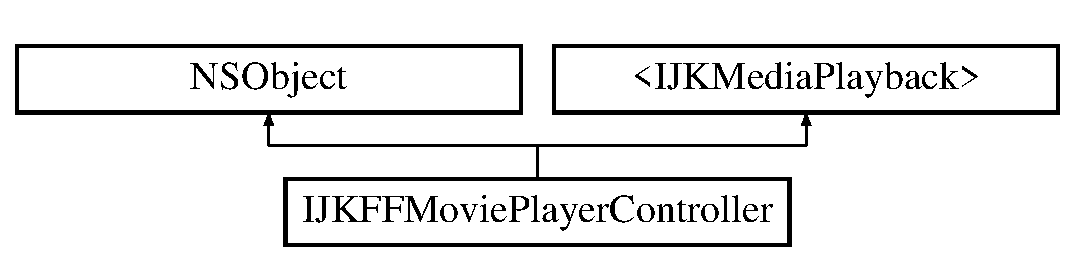
\includegraphics[height=2.000000cm]{interface_i_j_k_f_f_movie_player_controller}
\end{center}
\end{figure}
\subsection*{Instance Methods}
\begin{DoxyCompactItemize}
\item 
\mbox{\Hypertarget{interface_i_j_k_f_f_movie_player_controller_a43d3d3535b52972efab31668c6a31665}\label{interface_i_j_k_f_f_movie_player_controller_a43d3d3535b52972efab31668c6a31665}} 
(id) -\/ {\bfseries init\+With\+Content\+U\+R\+L\+:with\+Options\+:}
\item 
\mbox{\Hypertarget{interface_i_j_k_f_f_movie_player_controller_adead79aff8603127db86dfdc7c4dc720}\label{interface_i_j_k_f_f_movie_player_controller_adead79aff8603127db86dfdc7c4dc720}} 
(id) -\/ {\bfseries init\+With\+Content\+U\+R\+L\+String\+:with\+Options\+:}
\item 
\mbox{\Hypertarget{interface_i_j_k_f_f_movie_player_controller_aa913d429f90ea15adf9a1bb686a69d54}\label{interface_i_j_k_f_f_movie_player_controller_aa913d429f90ea15adf9a1bb686a69d54}} 
(void) -\/ {\bfseries prepare\+To\+Play}
\item 
\mbox{\Hypertarget{interface_i_j_k_f_f_movie_player_controller_ac72fd52394a2e0309d86fc4711870d30}\label{interface_i_j_k_f_f_movie_player_controller_ac72fd52394a2e0309d86fc4711870d30}} 
(void) -\/ {\bfseries play}
\item 
\mbox{\Hypertarget{interface_i_j_k_f_f_movie_player_controller_a2ff0f424c205d12bd66d0647e05aa545}\label{interface_i_j_k_f_f_movie_player_controller_a2ff0f424c205d12bd66d0647e05aa545}} 
(void) -\/ {\bfseries pause}
\item 
\mbox{\Hypertarget{interface_i_j_k_f_f_movie_player_controller_ace2b1458a9925420ddd3b06352b087c7}\label{interface_i_j_k_f_f_movie_player_controller_ace2b1458a9925420ddd3b06352b087c7}} 
(void) -\/ {\bfseries stop}
\item 
\mbox{\Hypertarget{interface_i_j_k_f_f_movie_player_controller_a81beb8077edb03f86b27031bbc25dc37}\label{interface_i_j_k_f_f_movie_player_controller_a81beb8077edb03f86b27031bbc25dc37}} 
(B\+O\+OL) -\/ {\bfseries is\+Playing}
\item 
\mbox{\Hypertarget{interface_i_j_k_f_f_movie_player_controller_a0078cdb6c28e907f9f72b56300f813cd}\label{interface_i_j_k_f_f_movie_player_controller_a0078cdb6c28e907f9f72b56300f813cd}} 
(long long) -\/ {\bfseries video\+Cached\+Packets}
\item 
\mbox{\Hypertarget{interface_i_j_k_f_f_movie_player_controller_a22a9e7c065a2ac8a00082216d1c44495}\label{interface_i_j_k_f_f_movie_player_controller_a22a9e7c065a2ac8a00082216d1c44495}} 
(long long) -\/ {\bfseries audio\+Cached\+Packets}
\item 
\mbox{\Hypertarget{interface_i_j_k_f_f_movie_player_controller_ab8e526bed501a6ade3f3efdfca917bc9}\label{interface_i_j_k_f_f_movie_player_controller_ab8e526bed501a6ade3f3efdfca917bc9}} 
(long long) -\/ {\bfseries video\+Cached\+Bytes}
\item 
\mbox{\Hypertarget{interface_i_j_k_f_f_movie_player_controller_a78e59821d7922785fd63f40b00dc0a23}\label{interface_i_j_k_f_f_movie_player_controller_a78e59821d7922785fd63f40b00dc0a23}} 
(long long) -\/ {\bfseries audio\+Cached\+Bytes}
\item 
\mbox{\Hypertarget{interface_i_j_k_f_f_movie_player_controller_a37f9ad05f54febcae66b77f13250b36f}\label{interface_i_j_k_f_f_movie_player_controller_a37f9ad05f54febcae66b77f13250b36f}} 
(long long) -\/ {\bfseries video\+Cached\+Duration}
\item 
\mbox{\Hypertarget{interface_i_j_k_f_f_movie_player_controller_a550267acd9c1c68d165d4f99d1f6f1b1}\label{interface_i_j_k_f_f_movie_player_controller_a550267acd9c1c68d165d4f99d1f6f1b1}} 
(long long) -\/ {\bfseries audio\+Cached\+Duration}
\item 
\mbox{\Hypertarget{interface_i_j_k_f_f_movie_player_controller_a8cb346259cf4e9b834547c6317aa365e}\label{interface_i_j_k_f_f_movie_player_controller_a8cb346259cf4e9b834547c6317aa365e}} 
(int64\+\_\+t) -\/ {\bfseries traffic\+Statistic}
\item 
\mbox{\Hypertarget{interface_i_j_k_f_f_movie_player_controller_ae14e92919551124ea568afd19d324bef}\label{interface_i_j_k_f_f_movie_player_controller_ae14e92919551124ea568afd19d324bef}} 
(float) -\/ {\bfseries drop\+Frame\+Rate}
\item 
\mbox{\Hypertarget{interface_i_j_k_f_f_movie_player_controller_a14c191a7a6940bdcef5891197c83bb98}\label{interface_i_j_k_f_f_movie_player_controller_a14c191a7a6940bdcef5891197c83bb98}} 
(void) -\/ {\bfseries set\+Pause\+In\+Background\+:}
\item 
\mbox{\Hypertarget{interface_i_j_k_f_f_movie_player_controller_ad3e00a607a03a1f40ccd8e5d5d50f9a0}\label{interface_i_j_k_f_f_movie_player_controller_ad3e00a607a03a1f40ccd8e5d5d50f9a0}} 
(B\+O\+OL) -\/ {\bfseries is\+Video\+Toolbox\+Open}
\item 
\mbox{\Hypertarget{interface_i_j_k_f_f_movie_player_controller_a14e520eed87804e211684197bb588479}\label{interface_i_j_k_f_f_movie_player_controller_a14e520eed87804e211684197bb588479}} 
(void) -\/ {\bfseries set\+Option\+Value\+:for\+Key\+:of\+Category\+:}
\item 
\mbox{\Hypertarget{interface_i_j_k_f_f_movie_player_controller_acae801b8fd75b680fedaa4cafadbfbce}\label{interface_i_j_k_f_f_movie_player_controller_acae801b8fd75b680fedaa4cafadbfbce}} 
(void) -\/ {\bfseries set\+Option\+Int\+Value\+:for\+Key\+:of\+Category\+:}
\item 
\mbox{\Hypertarget{interface_i_j_k_f_f_movie_player_controller_a1f557f146a72c41ad29a8bc0fe2b9c80}\label{interface_i_j_k_f_f_movie_player_controller_a1f557f146a72c41ad29a8bc0fe2b9c80}} 
(void) -\/ {\bfseries set\+Format\+Option\+Value\+:for\+Key\+:}
\item 
\mbox{\Hypertarget{interface_i_j_k_f_f_movie_player_controller_a646ae3d249cb465b807d8d9a28cf325c}\label{interface_i_j_k_f_f_movie_player_controller_a646ae3d249cb465b807d8d9a28cf325c}} 
(void) -\/ {\bfseries set\+Codec\+Option\+Value\+:for\+Key\+:}
\item 
\mbox{\Hypertarget{interface_i_j_k_f_f_movie_player_controller_ad8dbf07cd83ab166f5cf9ad17c220d68}\label{interface_i_j_k_f_f_movie_player_controller_ad8dbf07cd83ab166f5cf9ad17c220d68}} 
(void) -\/ {\bfseries set\+Sws\+Option\+Value\+:for\+Key\+:}
\item 
\mbox{\Hypertarget{interface_i_j_k_f_f_movie_player_controller_ac8424c80df33a71e421f1eb8978cab64}\label{interface_i_j_k_f_f_movie_player_controller_ac8424c80df33a71e421f1eb8978cab64}} 
(void) -\/ {\bfseries set\+Player\+Option\+Value\+:for\+Key\+:}
\item 
\mbox{\Hypertarget{interface_i_j_k_f_f_movie_player_controller_ae5738c9d7b390e47a7f79c431e3b90f4}\label{interface_i_j_k_f_f_movie_player_controller_ae5738c9d7b390e47a7f79c431e3b90f4}} 
(void) -\/ {\bfseries set\+Format\+Option\+Int\+Value\+:for\+Key\+:}
\item 
\mbox{\Hypertarget{interface_i_j_k_f_f_movie_player_controller_a6eed47c1b6c9e0a79fc198c3165cae3e}\label{interface_i_j_k_f_f_movie_player_controller_a6eed47c1b6c9e0a79fc198c3165cae3e}} 
(void) -\/ {\bfseries set\+Codec\+Option\+Int\+Value\+:for\+Key\+:}
\item 
\mbox{\Hypertarget{interface_i_j_k_f_f_movie_player_controller_ad7fa7842e87e670adde9d19a6bdb934a}\label{interface_i_j_k_f_f_movie_player_controller_ad7fa7842e87e670adde9d19a6bdb934a}} 
(void) -\/ {\bfseries set\+Sws\+Option\+Int\+Value\+:for\+Key\+:}
\item 
\mbox{\Hypertarget{interface_i_j_k_f_f_movie_player_controller_a126291ec24a1bbc42def39c02ec19410}\label{interface_i_j_k_f_f_movie_player_controller_a126291ec24a1bbc42def39c02ec19410}} 
(void) -\/ {\bfseries set\+Player\+Option\+Int\+Value\+:for\+Key\+:}
\item 
\mbox{\Hypertarget{interface_i_j_k_f_f_movie_player_controller_a745a9bd8677bf0ab47cf0f60cab6aa58}\label{interface_i_j_k_f_f_movie_player_controller_a745a9bd8677bf0ab47cf0f60cab6aa58}} 
(void) -\/ {\bfseries did\+Shutdown}
\end{DoxyCompactItemize}
\subsection*{Class Methods}
\begin{DoxyCompactItemize}
\item 
\mbox{\Hypertarget{interface_i_j_k_f_f_movie_player_controller_af5213a13ca0bd8dd13a81ee4764e8408}\label{interface_i_j_k_f_f_movie_player_controller_af5213a13ca0bd8dd13a81ee4764e8408}} 
(void) + {\bfseries set\+Log\+Report\+:}
\item 
\mbox{\Hypertarget{interface_i_j_k_f_f_movie_player_controller_a8fee9accc00e7593232174e0318a939a}\label{interface_i_j_k_f_f_movie_player_controller_a8fee9accc00e7593232174e0318a939a}} 
(void) + {\bfseries set\+Log\+Level\+:}
\item 
\mbox{\Hypertarget{interface_i_j_k_f_f_movie_player_controller_a2005c70e9ba3b7c41e499159b79d58dd}\label{interface_i_j_k_f_f_movie_player_controller_a2005c70e9ba3b7c41e499159b79d58dd}} 
(B\+O\+OL) + {\bfseries check\+If\+F\+Fmpeg\+Version\+Match\+:}
\item 
\mbox{\Hypertarget{interface_i_j_k_f_f_movie_player_controller_a78c99551cfce85f475776bfbeaa26d78}\label{interface_i_j_k_f_f_movie_player_controller_a78c99551cfce85f475776bfbeaa26d78}} 
(B\+O\+OL) + {\bfseries check\+If\+Player\+Version\+Match\+:version\+:}
\end{DoxyCompactItemize}
\subsection*{Properties}
\begin{DoxyCompactItemize}
\item 
\mbox{\Hypertarget{interface_i_j_k_f_f_movie_player_controller_a18679235448c8dcdf53923ff52f3996e}\label{interface_i_j_k_f_f_movie_player_controller_a18679235448c8dcdf53923ff52f3996e}} 
C\+G\+Float {\bfseries fps\+In\+Meta}
\item 
\mbox{\Hypertarget{interface_i_j_k_f_f_movie_player_controller_a0db0f235dcbd50f5c428d93da63102bc}\label{interface_i_j_k_f_f_movie_player_controller_a0db0f235dcbd50f5c428d93da63102bc}} 
C\+G\+Float {\bfseries fps\+At\+Output}
\item 
\mbox{\Hypertarget{interface_i_j_k_f_f_movie_player_controller_aed4abd7e53fabadb5248a03c25c2c6be}\label{interface_i_j_k_f_f_movie_player_controller_aed4abd7e53fabadb5248a03c25c2c6be}} 
B\+O\+OL {\bfseries should\+Show\+Hud\+View}
\item 
\mbox{\Hypertarget{interface_i_j_k_f_f_movie_player_controller_ae942312fae31898819931f17dc5491f3}\label{interface_i_j_k_f_f_movie_player_controller_ae942312fae31898819931f17dc5491f3}} 
id$<$ I\+J\+K\+Media\+Url\+Open\+Delegate $>$ {\bfseries segment\+Open\+Delegate}
\item 
\mbox{\Hypertarget{interface_i_j_k_f_f_movie_player_controller_a3701717b554cdfb233ae8e003ee36d07}\label{interface_i_j_k_f_f_movie_player_controller_a3701717b554cdfb233ae8e003ee36d07}} 
id$<$ I\+J\+K\+Media\+Url\+Open\+Delegate $>$ {\bfseries tcp\+Open\+Delegate}
\item 
\mbox{\Hypertarget{interface_i_j_k_f_f_movie_player_controller_a32d6776b77d5970a09874a66f6146c6c}\label{interface_i_j_k_f_f_movie_player_controller_a32d6776b77d5970a09874a66f6146c6c}} 
id$<$ I\+J\+K\+Media\+Url\+Open\+Delegate $>$ {\bfseries http\+Open\+Delegate}
\item 
\mbox{\Hypertarget{interface_i_j_k_f_f_movie_player_controller_a96d29e713101b63831b64fe9a726415c}\label{interface_i_j_k_f_f_movie_player_controller_a96d29e713101b63831b64fe9a726415c}} 
id$<$ I\+J\+K\+Media\+Url\+Open\+Delegate $>$ {\bfseries live\+Open\+Delegate}
\item 
\mbox{\Hypertarget{interface_i_j_k_f_f_movie_player_controller_aaf69dbfba1e393986ac9c90c538d93f5}\label{interface_i_j_k_f_f_movie_player_controller_aaf69dbfba1e393986ac9c90c538d93f5}} 
id$<$ I\+J\+K\+Media\+Native\+Invoke\+Delegate $>$ {\bfseries native\+Invoke\+Delegate}
\item 
\mbox{\Hypertarget{interface_i_j_k_f_f_movie_player_controller_af0fbac64e185a393f2c329d28b8af939}\label{interface_i_j_k_f_f_movie_player_controller_af0fbac64e185a393f2c329d28b8af939}} 
\hyperlink{interface_i_j_k_f_f_monitor}{I\+J\+K\+F\+F\+Monitor} $\ast$ {\bfseries monitor}
\end{DoxyCompactItemize}


The documentation for this class was generated from the following file\+:\begin{DoxyCompactItemize}
\item 
I\+J\+K\+F\+F\+Movie\+Player\+Controller.\+h\end{DoxyCompactItemize}

\hypertarget{interface_i_j_k_f_f_options}{}\section{I\+J\+K\+F\+F\+Options Class Reference}
\label{interface_i_j_k_f_f_options}\index{I\+J\+K\+F\+F\+Options@{I\+J\+K\+F\+F\+Options}}
Inheritance diagram for I\+J\+K\+F\+F\+Options\+:\begin{figure}[H]
\begin{center}
\leavevmode
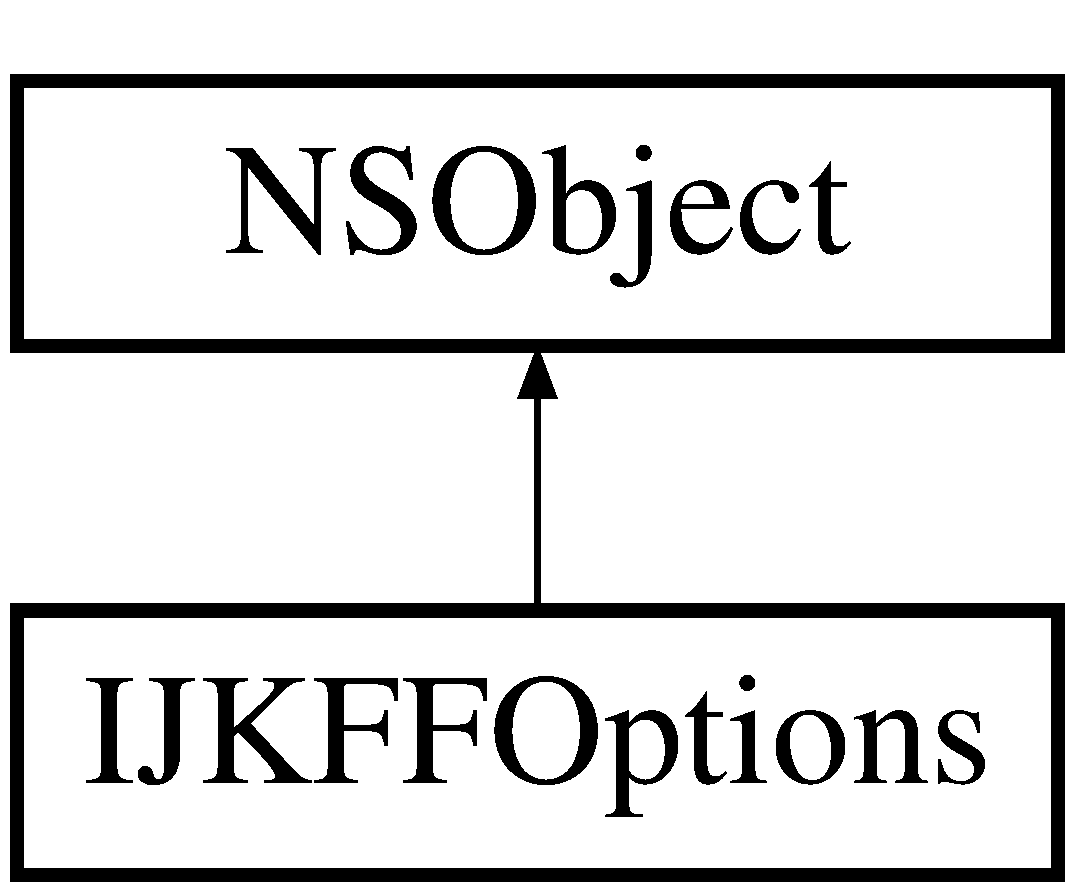
\includegraphics[height=2.000000cm]{interface_i_j_k_f_f_options}
\end{center}
\end{figure}
\subsection*{Instance Methods}
\begin{DoxyCompactItemize}
\item 
\mbox{\Hypertarget{interface_i_j_k_f_f_options_ae29f9f61780222bfb8c380736a0d5dcb}\label{interface_i_j_k_f_f_options_ae29f9f61780222bfb8c380736a0d5dcb}} 
(void) -\/ {\bfseries apply\+To\+:}
\item 
\mbox{\Hypertarget{interface_i_j_k_f_f_options_adc680e613d562f938d4e3d1ce13f602c}\label{interface_i_j_k_f_f_options_adc680e613d562f938d4e3d1ce13f602c}} 
(void) -\/ {\bfseries set\+Option\+Value\+:for\+Key\+:of\+Category\+:}
\item 
\mbox{\Hypertarget{interface_i_j_k_f_f_options_a2662ff6776b2e032c93c7a0ad25308a4}\label{interface_i_j_k_f_f_options_a2662ff6776b2e032c93c7a0ad25308a4}} 
(void) -\/ {\bfseries set\+Option\+Int\+Value\+:for\+Key\+:of\+Category\+:}
\item 
\mbox{\Hypertarget{interface_i_j_k_f_f_options_a4804c7696291b573fe5ed488a8e6f62e}\label{interface_i_j_k_f_f_options_a4804c7696291b573fe5ed488a8e6f62e}} 
(void) -\/ {\bfseries set\+Format\+Option\+Value\+:for\+Key\+:}
\item 
\mbox{\Hypertarget{interface_i_j_k_f_f_options_a69c4550c90152176c4752217a85a95a2}\label{interface_i_j_k_f_f_options_a69c4550c90152176c4752217a85a95a2}} 
(void) -\/ {\bfseries set\+Codec\+Option\+Value\+:for\+Key\+:}
\item 
\mbox{\Hypertarget{interface_i_j_k_f_f_options_a6e8685c995e629f567b8ae6e1dccb029}\label{interface_i_j_k_f_f_options_a6e8685c995e629f567b8ae6e1dccb029}} 
(void) -\/ {\bfseries set\+Sws\+Option\+Value\+:for\+Key\+:}
\item 
\mbox{\Hypertarget{interface_i_j_k_f_f_options_a5c3947f222ff9d5b5d431be5982e0620}\label{interface_i_j_k_f_f_options_a5c3947f222ff9d5b5d431be5982e0620}} 
(void) -\/ {\bfseries set\+Player\+Option\+Value\+:for\+Key\+:}
\item 
\mbox{\Hypertarget{interface_i_j_k_f_f_options_a045cd766bac666083d0350a30ea3e99a}\label{interface_i_j_k_f_f_options_a045cd766bac666083d0350a30ea3e99a}} 
(void) -\/ {\bfseries set\+Format\+Option\+Int\+Value\+:for\+Key\+:}
\item 
\mbox{\Hypertarget{interface_i_j_k_f_f_options_a9807f964a7c017fd51534b85a7f9d4c9}\label{interface_i_j_k_f_f_options_a9807f964a7c017fd51534b85a7f9d4c9}} 
(void) -\/ {\bfseries set\+Codec\+Option\+Int\+Value\+:for\+Key\+:}
\item 
\mbox{\Hypertarget{interface_i_j_k_f_f_options_a96a640d4e5d94eb9985c23394662da77}\label{interface_i_j_k_f_f_options_a96a640d4e5d94eb9985c23394662da77}} 
(void) -\/ {\bfseries set\+Sws\+Option\+Int\+Value\+:for\+Key\+:}
\item 
\mbox{\Hypertarget{interface_i_j_k_f_f_options_acb870477e8d099a10148e0bca3311995}\label{interface_i_j_k_f_f_options_acb870477e8d099a10148e0bca3311995}} 
(void) -\/ {\bfseries set\+Player\+Option\+Int\+Value\+:for\+Key\+:}
\end{DoxyCompactItemize}
\subsection*{Class Methods}
\begin{DoxyCompactItemize}
\item 
\mbox{\Hypertarget{interface_i_j_k_f_f_options_a5e6d820f1ade12c655f10fffff169989}\label{interface_i_j_k_f_f_options_a5e6d820f1ade12c655f10fffff169989}} 
(\hyperlink{interface_i_j_k_f_f_options}{I\+J\+K\+F\+F\+Options} $\ast$) + {\bfseries options\+By\+Default}
\end{DoxyCompactItemize}
\subsection*{Properties}
\begin{DoxyCompactItemize}
\item 
\mbox{\Hypertarget{interface_i_j_k_f_f_options_a2c256d81ca38f13c3fa8e28c4efa74aa}\label{interface_i_j_k_f_f_options_a2c256d81ca38f13c3fa8e28c4efa74aa}} 
B\+O\+OL {\bfseries show\+Hud\+View}
\end{DoxyCompactItemize}


The documentation for this class was generated from the following file\+:\begin{DoxyCompactItemize}
\item 
I\+J\+K\+F\+F\+Options.\+h\end{DoxyCompactItemize}

\hypertarget{interface_i_j_k_k_v_o_controller}{}\section{I\+J\+K\+K\+V\+O\+Controller Class Reference}
\label{interface_i_j_k_k_v_o_controller}\index{I\+J\+K\+K\+V\+O\+Controller@{I\+J\+K\+K\+V\+O\+Controller}}
Inheritance diagram for I\+J\+K\+K\+V\+O\+Controller\+:\begin{figure}[H]
\begin{center}
\leavevmode
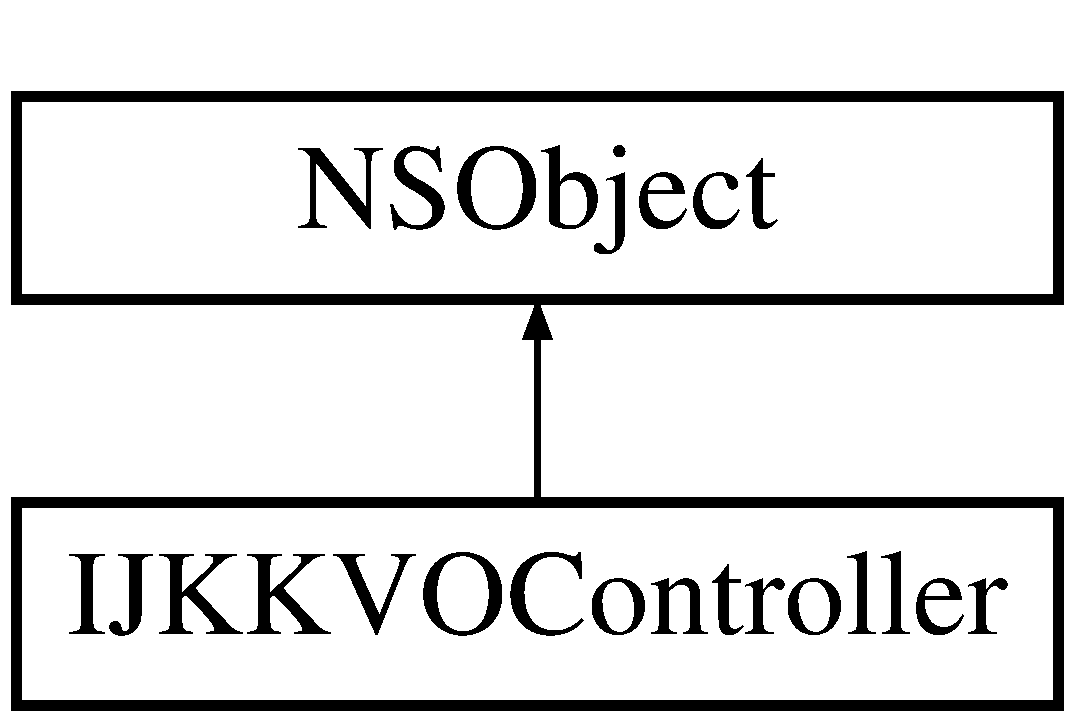
\includegraphics[height=2.000000cm]{interface_i_j_k_k_v_o_controller}
\end{center}
\end{figure}
\subsection*{Instance Methods}
\begin{DoxyCompactItemize}
\item 
\mbox{\Hypertarget{interface_i_j_k_k_v_o_controller_ae20030eb76b02f1d6b4c0af238385feb}\label{interface_i_j_k_k_v_o_controller_ae20030eb76b02f1d6b4c0af238385feb}} 
(id) -\/ {\bfseries init\+With\+Target\+:}
\item 
\mbox{\Hypertarget{interface_i_j_k_k_v_o_controller_afc65b1c9d1cdd9e175f7f49114760dbe}\label{interface_i_j_k_k_v_o_controller_afc65b1c9d1cdd9e175f7f49114760dbe}} 
(void) -\/ {\bfseries safely\+Add\+Observer\+:for\+Key\+Path\+:options\+:context\+:}
\item 
\mbox{\Hypertarget{interface_i_j_k_k_v_o_controller_a672f4972a2aedc6386c563127210571f}\label{interface_i_j_k_k_v_o_controller_a672f4972a2aedc6386c563127210571f}} 
(void) -\/ {\bfseries safely\+Remove\+Observer\+:for\+Key\+Path\+:}
\item 
\mbox{\Hypertarget{interface_i_j_k_k_v_o_controller_a99dccbac8f018dc3e727c4d70c611003}\label{interface_i_j_k_k_v_o_controller_a99dccbac8f018dc3e727c4d70c611003}} 
(void) -\/ {\bfseries safely\+Remove\+All\+Observers}
\end{DoxyCompactItemize}


The documentation for this class was generated from the following file\+:\begin{DoxyCompactItemize}
\item 
I\+J\+K\+K\+V\+O\+Controller.\+h\end{DoxyCompactItemize}

\hypertarget{interface_i_j_k_media_module}{}\section{I\+J\+K\+Media\+Module Class Reference}
\label{interface_i_j_k_media_module}\index{I\+J\+K\+Media\+Module@{I\+J\+K\+Media\+Module}}
Inheritance diagram for I\+J\+K\+Media\+Module\+:\begin{figure}[H]
\begin{center}
\leavevmode
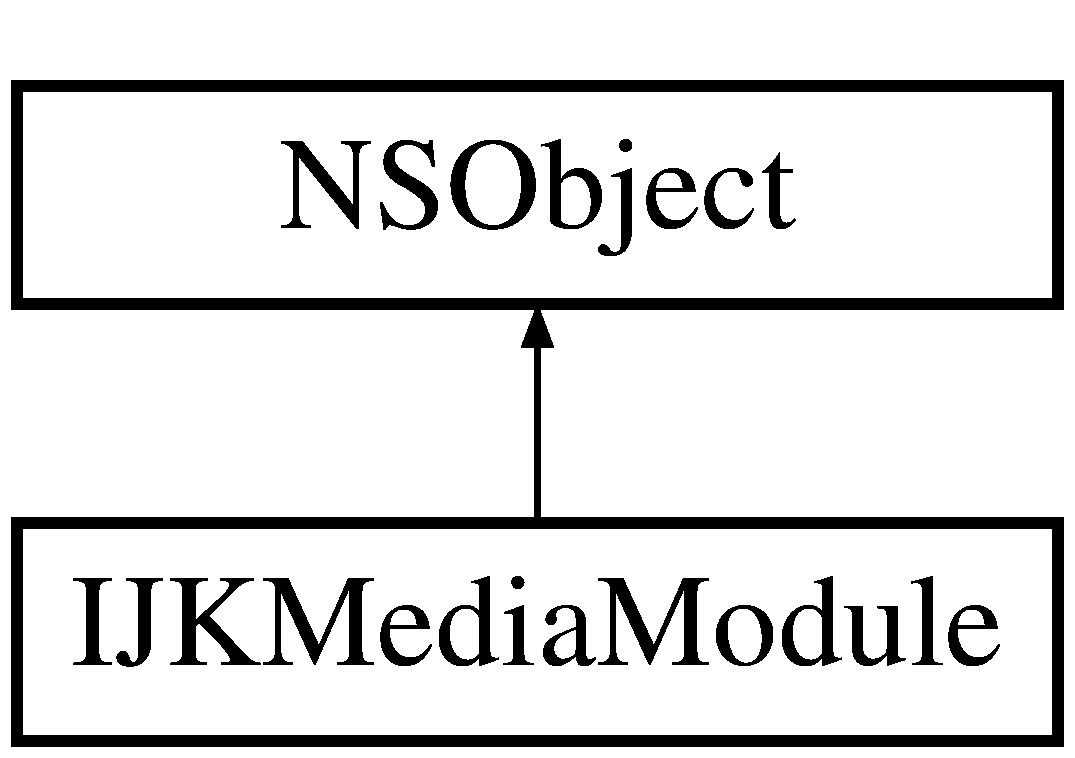
\includegraphics[height=2.000000cm]{interface_i_j_k_media_module}
\end{center}
\end{figure}
\subsection*{Class Methods}
\begin{DoxyCompactItemize}
\item 
\mbox{\Hypertarget{interface_i_j_k_media_module_a0c749d2c2a13bfeb408502f9d18a5cca}\label{interface_i_j_k_media_module_a0c749d2c2a13bfeb408502f9d18a5cca}} 
(\hyperlink{interface_i_j_k_media_module}{I\+J\+K\+Media\+Module} $\ast$) + {\bfseries shared\+Module}
\end{DoxyCompactItemize}
\subsection*{Properties}
\begin{DoxyCompactItemize}
\item 
\mbox{\Hypertarget{interface_i_j_k_media_module_ad080b2121247de7d6fe706053f7f25df}\label{interface_i_j_k_media_module_ad080b2121247de7d6fe706053f7f25df}} 
B\+O\+OL {\bfseries app\+Idle\+Timer\+Disabled}
\item 
\mbox{\Hypertarget{interface_i_j_k_media_module_a2bbe08dfd29afee83d8b232f286f27e1}\label{interface_i_j_k_media_module_a2bbe08dfd29afee83d8b232f286f27e1}} 
B\+O\+OL {\bfseries media\+Module\+Idle\+Timer\+Disabled}
\end{DoxyCompactItemize}


The documentation for this class was generated from the following file\+:\begin{DoxyCompactItemize}
\item 
I\+J\+K\+Media\+Module.\+h\end{DoxyCompactItemize}

\hypertarget{protocol_i_j_k_media_native_invoke_delegate_01-p}{}\section{$<$I\+J\+K\+Media\+Native\+Invoke\+Delegate $>$ Protocol Reference}
\label{protocol_i_j_k_media_native_invoke_delegate_01-p}\index{$<$\+I\+J\+K\+Media\+Native\+Invoke\+Delegate $>$@{$<$\+I\+J\+K\+Media\+Native\+Invoke\+Delegate $>$}}
Inheritance diagram for $<$I\+J\+K\+Media\+Native\+Invoke\+Delegate $>$\+:\begin{figure}[H]
\begin{center}
\leavevmode
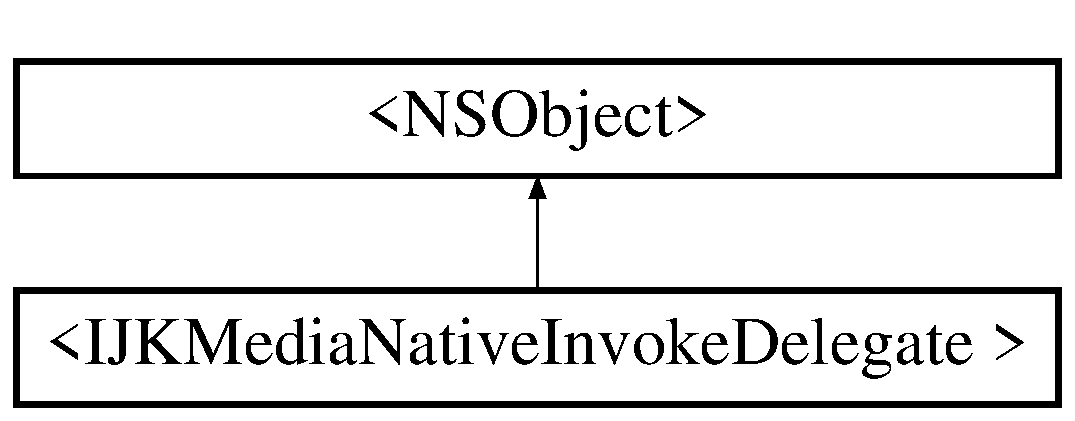
\includegraphics[height=2.000000cm]{protocol_i_j_k_media_native_invoke_delegate_01-p}
\end{center}
\end{figure}
\subsection*{Instance Methods}
\begin{DoxyCompactItemize}
\item 
\mbox{\Hypertarget{protocol_i_j_k_media_native_invoke_delegate_01-p_a7e88e4e115c899a5d26999cd46e99d21}\label{protocol_i_j_k_media_native_invoke_delegate_01-p_a7e88e4e115c899a5d26999cd46e99d21}} 
(int) -\/ {\bfseries invoke\+:attributes\+:}
\end{DoxyCompactItemize}


The documentation for this protocol was generated from the following file\+:\begin{DoxyCompactItemize}
\item 
I\+J\+K\+Media\+Playback.\+h\end{DoxyCompactItemize}

\hypertarget{protocol_i_j_k_media_playback_01-p}{}\section{$<$I\+J\+K\+Media\+Playback $>$ Protocol Reference}
\label{protocol_i_j_k_media_playback_01-p}\index{$<$\+I\+J\+K\+Media\+Playback $>$@{$<$\+I\+J\+K\+Media\+Playback $>$}}
Inheritance diagram for $<$I\+J\+K\+Media\+Playback $>$\+:\begin{figure}[H]
\begin{center}
\leavevmode
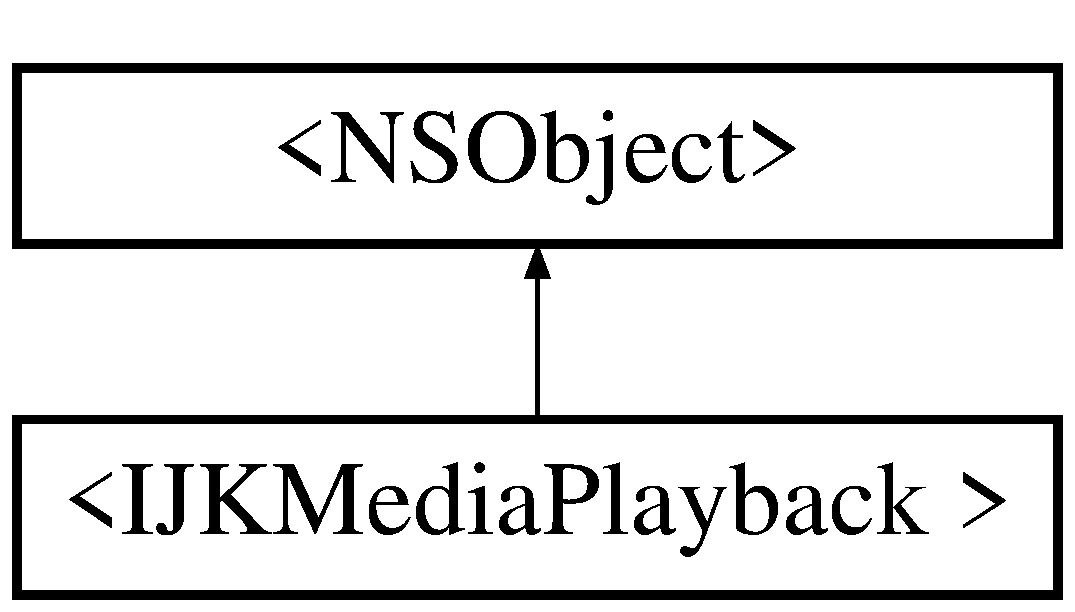
\includegraphics[height=2.000000cm]{protocol_i_j_k_media_playback_01-p}
\end{center}
\end{figure}
\subsection*{Instance Methods}
\begin{DoxyCompactItemize}
\item 
\mbox{\Hypertarget{protocol_i_j_k_media_playback_01-p_a5f8327e47f7be52883f1713131d43a55}\label{protocol_i_j_k_media_playback_01-p_a5f8327e47f7be52883f1713131d43a55}} 
(void) -\/ {\bfseries prepare\+To\+Play}
\item 
\mbox{\Hypertarget{protocol_i_j_k_media_playback_01-p_a1f846d175d10afed87bd9554c199c2b3}\label{protocol_i_j_k_media_playback_01-p_a1f846d175d10afed87bd9554c199c2b3}} 
(void) -\/ {\bfseries play}
\item 
\mbox{\Hypertarget{protocol_i_j_k_media_playback_01-p_aa5b270d9c1eee031b0e36d42f40d7daa}\label{protocol_i_j_k_media_playback_01-p_aa5b270d9c1eee031b0e36d42f40d7daa}} 
(void) -\/ {\bfseries pause}
\item 
\mbox{\Hypertarget{protocol_i_j_k_media_playback_01-p_a6a52157b65b3882756bf2f815a2fd6c2}\label{protocol_i_j_k_media_playback_01-p_a6a52157b65b3882756bf2f815a2fd6c2}} 
(void) -\/ {\bfseries stop}
\item 
\mbox{\Hypertarget{protocol_i_j_k_media_playback_01-p_a8a4545b217adb6c2c1600728149e6f38}\label{protocol_i_j_k_media_playback_01-p_a8a4545b217adb6c2c1600728149e6f38}} 
(B\+O\+OL) -\/ {\bfseries is\+Playing}
\item 
\mbox{\Hypertarget{protocol_i_j_k_media_playback_01-p_aeddfe26e15aada7d172a3ab074960162}\label{protocol_i_j_k_media_playback_01-p_aeddfe26e15aada7d172a3ab074960162}} 
(void) -\/ {\bfseries shutdown}
\item 
\mbox{\Hypertarget{protocol_i_j_k_media_playback_01-p_aa3b178c08d4c1167363661c069a06d8d}\label{protocol_i_j_k_media_playback_01-p_aa3b178c08d4c1167363661c069a06d8d}} 
(void) -\/ {\bfseries set\+Pause\+In\+Background\+:}
\item 
\mbox{\Hypertarget{protocol_i_j_k_media_playback_01-p_a15b3df4070f1b4a299473ed8d82ae8e2}\label{protocol_i_j_k_media_playback_01-p_a15b3df4070f1b4a299473ed8d82ae8e2}} 
(U\+I\+Image $\ast$) -\/ {\bfseries thumbnail\+Image\+At\+Current\+Time}
\end{DoxyCompactItemize}
\subsection*{Public Attributes}
\begin{DoxyCompactItemize}
\item 
\mbox{\Hypertarget{protocol_i_j_k_media_playback_01-p_a5721c242f9e2de9e35617b982878f41c}\label{protocol_i_j_k_media_playback_01-p_a5721c242f9e2de9e35617b982878f41c}} 
I\+J\+K\+\_\+\+E\+X\+T\+E\+RN N\+S\+String $\ast$const {\bfseries I\+J\+K\+M\+P\+Media\+Playback\+Is\+Prepared\+To\+Play\+Did\+Change\+Notification}
\item 
\mbox{\Hypertarget{protocol_i_j_k_media_playback_01-p_a10fc1ef805fb39c16b51b1abd81d12c8}\label{protocol_i_j_k_media_playback_01-p_a10fc1ef805fb39c16b51b1abd81d12c8}} 
I\+J\+K\+\_\+\+E\+X\+T\+E\+RN N\+S\+String $\ast$const {\bfseries I\+J\+K\+M\+P\+Movie\+Player\+Scaling\+Mode\+Did\+Change\+Notification}
\item 
\mbox{\Hypertarget{protocol_i_j_k_media_playback_01-p_ab55aa2dd70bf74e486851972bf5c326a}\label{protocol_i_j_k_media_playback_01-p_ab55aa2dd70bf74e486851972bf5c326a}} 
I\+J\+K\+\_\+\+E\+X\+T\+E\+RN N\+S\+String $\ast$const {\bfseries I\+J\+K\+M\+P\+Movie\+Player\+Playback\+Did\+Finish\+Notification}
\item 
\mbox{\Hypertarget{protocol_i_j_k_media_playback_01-p_a96f0c97d65c2cfa69bcfda2b4c8f0f4b}\label{protocol_i_j_k_media_playback_01-p_a96f0c97d65c2cfa69bcfda2b4c8f0f4b}} 
I\+J\+K\+\_\+\+E\+X\+T\+E\+RN N\+S\+String $\ast$const {\bfseries I\+J\+K\+M\+P\+Movie\+Player\+Playback\+Did\+Finish\+Reason\+User\+Info\+Key}
\item 
\mbox{\Hypertarget{protocol_i_j_k_media_playback_01-p_a114cdde557af7aa34c954f38ffe1abe5}\label{protocol_i_j_k_media_playback_01-p_a114cdde557af7aa34c954f38ffe1abe5}} 
I\+J\+K\+\_\+\+E\+X\+T\+E\+RN N\+S\+String $\ast$const {\bfseries I\+J\+K\+M\+P\+Movie\+Player\+Playback\+State\+Did\+Change\+Notification}
\item 
\mbox{\Hypertarget{protocol_i_j_k_media_playback_01-p_a3fa9869fd6ac033ed8de4c90305ec538}\label{protocol_i_j_k_media_playback_01-p_a3fa9869fd6ac033ed8de4c90305ec538}} 
I\+J\+K\+\_\+\+E\+X\+T\+E\+RN N\+S\+String $\ast$const {\bfseries I\+J\+K\+M\+P\+Movie\+Player\+Load\+State\+Did\+Change\+Notification}
\item 
\mbox{\Hypertarget{protocol_i_j_k_media_playback_01-p_adbb21e80c80f0f8649f0e25a02d1ffbd}\label{protocol_i_j_k_media_playback_01-p_adbb21e80c80f0f8649f0e25a02d1ffbd}} 
I\+J\+K\+\_\+\+E\+X\+T\+E\+RN N\+S\+String $\ast$const {\bfseries I\+J\+K\+M\+P\+Movie\+Player\+Is\+Air\+Play\+Video\+Active\+Did\+Change\+Notification}
\item 
\mbox{\Hypertarget{protocol_i_j_k_media_playback_01-p_a9a971c9d3a8043fea32f51a30e9d5435}\label{protocol_i_j_k_media_playback_01-p_a9a971c9d3a8043fea32f51a30e9d5435}} 
I\+J\+K\+\_\+\+E\+X\+T\+E\+RN N\+S\+String $\ast$const {\bfseries I\+J\+K\+M\+P\+Movie\+Natural\+Size\+Available\+Notification}
\item 
\mbox{\Hypertarget{protocol_i_j_k_media_playback_01-p_aff4a50df43c4b692e1275cdee3fb3f2c}\label{protocol_i_j_k_media_playback_01-p_aff4a50df43c4b692e1275cdee3fb3f2c}} 
I\+J\+K\+\_\+\+E\+X\+T\+E\+RN N\+S\+String $\ast$const {\bfseries I\+J\+K\+M\+P\+Movie\+Player\+Video\+Decoder\+Open\+Notification}
\item 
\mbox{\Hypertarget{protocol_i_j_k_media_playback_01-p_a885ddeb23420bfe3c6b9007b6770943d}\label{protocol_i_j_k_media_playback_01-p_a885ddeb23420bfe3c6b9007b6770943d}} 
I\+J\+K\+\_\+\+E\+X\+T\+E\+RN N\+S\+String $\ast$const {\bfseries I\+J\+K\+M\+P\+Movie\+Player\+First\+Video\+Frame\+Rendered\+Notification}
\item 
\mbox{\Hypertarget{protocol_i_j_k_media_playback_01-p_aaf1f139d7a9a94105a54e2d962686aae}\label{protocol_i_j_k_media_playback_01-p_aaf1f139d7a9a94105a54e2d962686aae}} 
I\+J\+K\+\_\+\+E\+X\+T\+E\+RN N\+S\+String $\ast$const {\bfseries I\+J\+K\+M\+P\+Movie\+Player\+First\+Audio\+Frame\+Rendered\+Notification}
\item 
\mbox{\Hypertarget{protocol_i_j_k_media_playback_01-p_ad84d181aa6a5233aa74b84a825484ddf}\label{protocol_i_j_k_media_playback_01-p_ad84d181aa6a5233aa74b84a825484ddf}} 
I\+J\+K\+\_\+\+E\+X\+T\+E\+RN N\+S\+String $\ast$const {\bfseries I\+J\+K\+M\+P\+Movie\+Player\+Did\+Seek\+Complete\+Notification}
\item 
\mbox{\Hypertarget{protocol_i_j_k_media_playback_01-p_a7d3cd42c54b2f723e3e4ec6e47dd4e5f}\label{protocol_i_j_k_media_playback_01-p_a7d3cd42c54b2f723e3e4ec6e47dd4e5f}} 
I\+J\+K\+\_\+\+E\+X\+T\+E\+RN N\+S\+String $\ast$const {\bfseries I\+J\+K\+M\+P\+Movie\+Player\+Did\+Seek\+Complete\+Target\+Key}
\item 
\mbox{\Hypertarget{protocol_i_j_k_media_playback_01-p_a26a594b91470868fa9fa797458df35bd}\label{protocol_i_j_k_media_playback_01-p_a26a594b91470868fa9fa797458df35bd}} 
I\+J\+K\+\_\+\+E\+X\+T\+E\+RN N\+S\+String $\ast$const {\bfseries I\+J\+K\+M\+P\+Movie\+Player\+Did\+Seek\+Complete\+Error\+Key}
\item 
\mbox{\Hypertarget{protocol_i_j_k_media_playback_01-p_ae048a741e323554a74360aac444a962e}\label{protocol_i_j_k_media_playback_01-p_ae048a741e323554a74360aac444a962e}} 
I\+J\+K\+\_\+\+E\+X\+T\+E\+RN N\+S\+String $\ast$const {\bfseries I\+J\+K\+M\+P\+Movie\+Player\+Did\+Accurate\+Seek\+Complete\+Cur\+Pos}
\item 
\mbox{\Hypertarget{protocol_i_j_k_media_playback_01-p_a7b5ce43c9585d95aa01b15d8926d3108}\label{protocol_i_j_k_media_playback_01-p_a7b5ce43c9585d95aa01b15d8926d3108}} 
I\+J\+K\+\_\+\+E\+X\+T\+E\+RN N\+S\+String $\ast$const {\bfseries I\+J\+K\+M\+P\+Movie\+Player\+Accurate\+Seek\+Complete\+Notification}
\end{DoxyCompactItemize}
\subsection*{Properties}
\begin{DoxyCompactItemize}
\item 
\mbox{\Hypertarget{protocol_i_j_k_media_playback_01-p_aef76aae5b5efb65b8f6b98dda1100f4d}\label{protocol_i_j_k_media_playback_01-p_aef76aae5b5efb65b8f6b98dda1100f4d}} 
U\+I\+View $\ast$ {\bfseries view}
\item 
\mbox{\Hypertarget{protocol_i_j_k_media_playback_01-p_a5b90d326e59a335400edd7c0c9bb8d00}\label{protocol_i_j_k_media_playback_01-p_a5b90d326e59a335400edd7c0c9bb8d00}} 
N\+S\+Time\+Interval {\bfseries current\+Playback\+Time}
\item 
\mbox{\Hypertarget{protocol_i_j_k_media_playback_01-p_af27a6f256db2d0d9e26401a9d06ed267}\label{protocol_i_j_k_media_playback_01-p_af27a6f256db2d0d9e26401a9d06ed267}} 
N\+S\+Time\+Interval {\bfseries duration}
\item 
\mbox{\Hypertarget{protocol_i_j_k_media_playback_01-p_a3ad5ebd19d7667836f2148d83dd34b27}\label{protocol_i_j_k_media_playback_01-p_a3ad5ebd19d7667836f2148d83dd34b27}} 
N\+S\+Time\+Interval {\bfseries playable\+Duration}
\item 
\mbox{\Hypertarget{protocol_i_j_k_media_playback_01-p_a2e57462ca61aac198bcf4c300d26cdb2}\label{protocol_i_j_k_media_playback_01-p_a2e57462ca61aac198bcf4c300d26cdb2}} 
N\+S\+Integer {\bfseries buffering\+Progress}
\item 
\mbox{\Hypertarget{protocol_i_j_k_media_playback_01-p_a8df2d5c5cb44d415dcecbe9838e2c052}\label{protocol_i_j_k_media_playback_01-p_a8df2d5c5cb44d415dcecbe9838e2c052}} 
B\+O\+OL {\bfseries is\+Prepared\+To\+Play}
\item 
\mbox{\Hypertarget{protocol_i_j_k_media_playback_01-p_a4ee11444f52ccbed97ca6870bd44f6c6}\label{protocol_i_j_k_media_playback_01-p_a4ee11444f52ccbed97ca6870bd44f6c6}} 
I\+J\+K\+M\+P\+Movie\+Playback\+State {\bfseries playback\+State}
\item 
\mbox{\Hypertarget{protocol_i_j_k_media_playback_01-p_a1fcff4a12a4a4db4aaa4c0017e1d35c4}\label{protocol_i_j_k_media_playback_01-p_a1fcff4a12a4a4db4aaa4c0017e1d35c4}} 
I\+J\+K\+M\+P\+Movie\+Load\+State {\bfseries load\+State}
\item 
\mbox{\Hypertarget{protocol_i_j_k_media_playback_01-p_af0842a80d570e065b6199f948219dfca}\label{protocol_i_j_k_media_playback_01-p_af0842a80d570e065b6199f948219dfca}} 
int64\+\_\+t {\bfseries number\+Of\+Bytes\+Transferred}
\item 
\mbox{\Hypertarget{protocol_i_j_k_media_playback_01-p_a6c77c9d7c4ff98f8e9f02b8de0bdcf6f}\label{protocol_i_j_k_media_playback_01-p_a6c77c9d7c4ff98f8e9f02b8de0bdcf6f}} 
C\+G\+Size {\bfseries natural\+Size}
\item 
\mbox{\Hypertarget{protocol_i_j_k_media_playback_01-p_abb32f282e57276d2659c50ad40552fb7}\label{protocol_i_j_k_media_playback_01-p_abb32f282e57276d2659c50ad40552fb7}} 
I\+J\+K\+M\+P\+Movie\+Scaling\+Mode {\bfseries scaling\+Mode}
\item 
\mbox{\Hypertarget{protocol_i_j_k_media_playback_01-p_a70a9bad5e0e00a8d467c05f1bd876ca1}\label{protocol_i_j_k_media_playback_01-p_a70a9bad5e0e00a8d467c05f1bd876ca1}} 
B\+O\+OL {\bfseries should\+Autoplay}
\item 
\mbox{\Hypertarget{protocol_i_j_k_media_playback_01-p_ac8405ac042bbdf06b85e4cbf845b7b55}\label{protocol_i_j_k_media_playback_01-p_ac8405ac042bbdf06b85e4cbf845b7b55}} 
B\+O\+OL {\bfseries allows\+Media\+Air\+Play}
\item 
\mbox{\Hypertarget{protocol_i_j_k_media_playback_01-p_abf2723f068b04a32eff5511827184d39}\label{protocol_i_j_k_media_playback_01-p_abf2723f068b04a32eff5511827184d39}} 
B\+O\+OL {\bfseries is\+Danmaku\+Media\+Air\+Play}
\item 
\mbox{\Hypertarget{protocol_i_j_k_media_playback_01-p_ac75a338858a3763465cbbc9c60fd8c57}\label{protocol_i_j_k_media_playback_01-p_ac75a338858a3763465cbbc9c60fd8c57}} 
B\+O\+OL {\bfseries air\+Play\+Media\+Active}
\item 
\mbox{\Hypertarget{protocol_i_j_k_media_playback_01-p_a835ad839e3fadfdec7c1ed3ce6cd74c1}\label{protocol_i_j_k_media_playback_01-p_a835ad839e3fadfdec7c1ed3ce6cd74c1}} 
float {\bfseries playback\+Rate}
\item 
\mbox{\Hypertarget{protocol_i_j_k_media_playback_01-p_a38de13f96b636f26183ce8b4abc45f16}\label{protocol_i_j_k_media_playback_01-p_a38de13f96b636f26183ce8b4abc45f16}} 
float {\bfseries playback\+Volume}
\end{DoxyCompactItemize}


The documentation for this protocol was generated from the following file\+:\begin{DoxyCompactItemize}
\item 
I\+J\+K\+Media\+Playback.\+h\end{DoxyCompactItemize}

\hypertarget{interface_i_j_k_media_url_open_data}{}\section{I\+J\+K\+Media\+Url\+Open\+Data Class Reference}
\label{interface_i_j_k_media_url_open_data}\index{I\+J\+K\+Media\+Url\+Open\+Data@{I\+J\+K\+Media\+Url\+Open\+Data}}
Inheritance diagram for I\+J\+K\+Media\+Url\+Open\+Data\+:\begin{figure}[H]
\begin{center}
\leavevmode
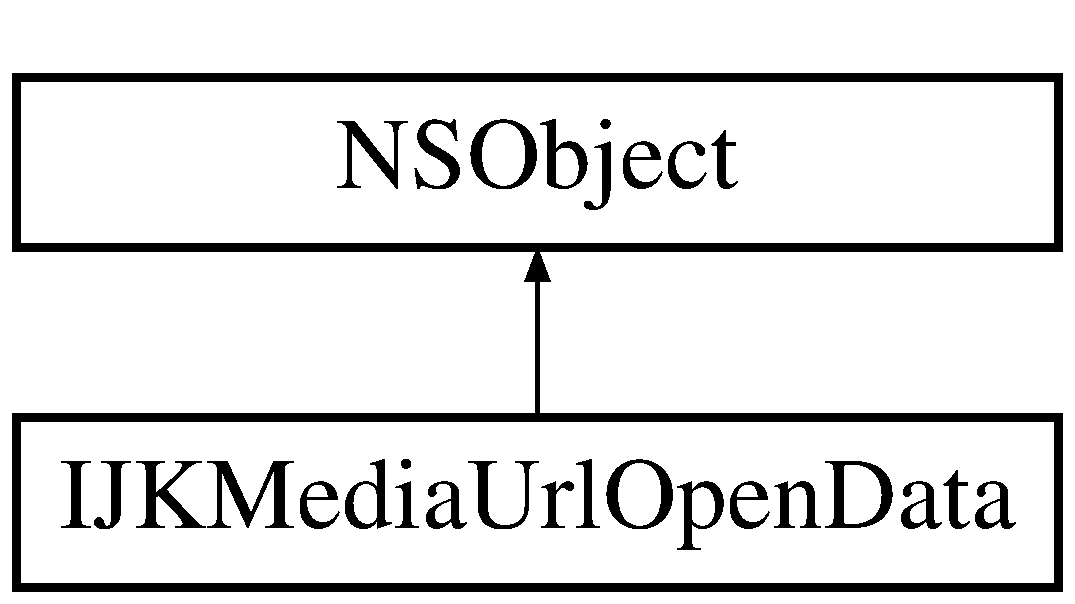
\includegraphics[height=2.000000cm]{interface_i_j_k_media_url_open_data}
\end{center}
\end{figure}
\subsection*{Instance Methods}
\begin{DoxyCompactItemize}
\item 
\mbox{\Hypertarget{interface_i_j_k_media_url_open_data_aebc5e26eeee34eaeb6ce7355c57674e4}\label{interface_i_j_k_media_url_open_data_aebc5e26eeee34eaeb6ce7355c57674e4}} 
(id) -\/ {\bfseries init\+With\+Url\+:event\+:segment\+Index\+:retry\+Counter\+:}
\end{DoxyCompactItemize}
\subsection*{Properties}
\begin{DoxyCompactItemize}
\item 
\mbox{\Hypertarget{interface_i_j_k_media_url_open_data_a719982e2ba62c975f6fd5068ea294bdb}\label{interface_i_j_k_media_url_open_data_a719982e2ba62c975f6fd5068ea294bdb}} 
I\+J\+K\+Media\+Event {\bfseries event}
\item 
\mbox{\Hypertarget{interface_i_j_k_media_url_open_data_a5d7a6513b91b11dfb4ce46dc46c65e5f}\label{interface_i_j_k_media_url_open_data_a5d7a6513b91b11dfb4ce46dc46c65e5f}} 
int {\bfseries segment\+Index}
\item 
\mbox{\Hypertarget{interface_i_j_k_media_url_open_data_a12b71044ef4241f200e3dbfdd4ecb860}\label{interface_i_j_k_media_url_open_data_a12b71044ef4241f200e3dbfdd4ecb860}} 
int {\bfseries retry\+Counter}
\item 
\mbox{\Hypertarget{interface_i_j_k_media_url_open_data_a71ca433dfbf6f2f92e84e8a593ec087d}\label{interface_i_j_k_media_url_open_data_a71ca433dfbf6f2f92e84e8a593ec087d}} 
N\+S\+String $\ast$ {\bfseries url}
\item 
\mbox{\Hypertarget{interface_i_j_k_media_url_open_data_a6c41e8bf2234a3a7d34af7411b36b67e}\label{interface_i_j_k_media_url_open_data_a6c41e8bf2234a3a7d34af7411b36b67e}} 
int {\bfseries fd}
\item 
\mbox{\Hypertarget{interface_i_j_k_media_url_open_data_a6757fbf435294441d556e10f12827804}\label{interface_i_j_k_media_url_open_data_a6757fbf435294441d556e10f12827804}} 
N\+S\+String $\ast$ {\bfseries msg}
\item 
\mbox{\Hypertarget{interface_i_j_k_media_url_open_data_ae5add1589d9bf626cf7351118f3463b7}\label{interface_i_j_k_media_url_open_data_ae5add1589d9bf626cf7351118f3463b7}} 
int {\bfseries error}
\item 
\mbox{\Hypertarget{interface_i_j_k_media_url_open_data_a34cfabdf5dece81bd245110e1d07e40e}\label{interface_i_j_k_media_url_open_data_a34cfabdf5dece81bd245110e1d07e40e}} 
B\+O\+OL {\bfseries handled}
\item 
\mbox{\Hypertarget{interface_i_j_k_media_url_open_data_a9b44cd5d701744e02bd4eeabf2be6379}\label{interface_i_j_k_media_url_open_data_a9b44cd5d701744e02bd4eeabf2be6379}} 
B\+O\+OL {\bfseries url\+Changed}
\end{DoxyCompactItemize}


The documentation for this class was generated from the following file\+:\begin{DoxyCompactItemize}
\item 
I\+J\+K\+Media\+Playback.\+h\end{DoxyCompactItemize}

\hypertarget{protocol_i_j_k_media_url_open_delegate_01-p}{}\section{$<$I\+J\+K\+Media\+Url\+Open\+Delegate $>$ Protocol Reference}
\label{protocol_i_j_k_media_url_open_delegate_01-p}\index{$<$\+I\+J\+K\+Media\+Url\+Open\+Delegate $>$@{$<$\+I\+J\+K\+Media\+Url\+Open\+Delegate $>$}}
Inheritance diagram for $<$I\+J\+K\+Media\+Url\+Open\+Delegate $>$\+:\begin{figure}[H]
\begin{center}
\leavevmode
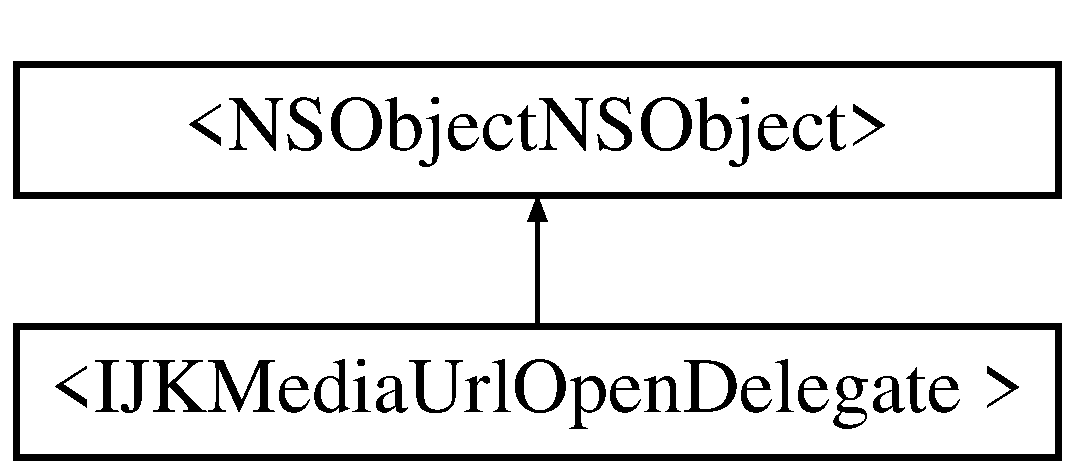
\includegraphics[height=2.000000cm]{protocol_i_j_k_media_url_open_delegate_01-p}
\end{center}
\end{figure}
\subsection*{Instance Methods}
\begin{DoxyCompactItemize}
\item 
\mbox{\Hypertarget{protocol_i_j_k_media_url_open_delegate_01-p_a35bc54d1974b670290ac96cd857a21f5}\label{protocol_i_j_k_media_url_open_delegate_01-p_a35bc54d1974b670290ac96cd857a21f5}} 
(void) -\/ {\bfseries will\+Open\+Url\+:}
\end{DoxyCompactItemize}


The documentation for this protocol was generated from the following file\+:\begin{DoxyCompactItemize}
\item 
I\+J\+K\+Media\+Playback.\+h\end{DoxyCompactItemize}

\hypertarget{interface_i_j_k_m_p_movie_player_controller}{}\section{I\+J\+K\+M\+P\+Movie\+Player\+Controller Class Reference}
\label{interface_i_j_k_m_p_movie_player_controller}\index{I\+J\+K\+M\+P\+Movie\+Player\+Controller@{I\+J\+K\+M\+P\+Movie\+Player\+Controller}}
Inheritance diagram for I\+J\+K\+M\+P\+Movie\+Player\+Controller\+:\begin{figure}[H]
\begin{center}
\leavevmode
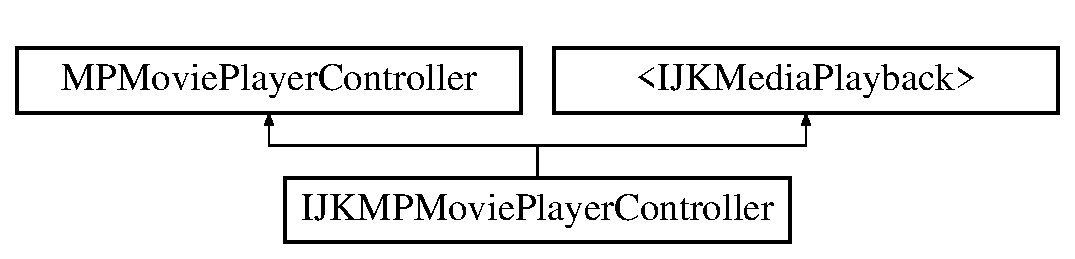
\includegraphics[height=2.000000cm]{interface_i_j_k_m_p_movie_player_controller}
\end{center}
\end{figure}
\subsection*{Instance Methods}
\begin{DoxyCompactItemize}
\item 
\mbox{\Hypertarget{interface_i_j_k_m_p_movie_player_controller_a6adcc4d43ff855cefc43a110b8f2511b}\label{interface_i_j_k_m_p_movie_player_controller_a6adcc4d43ff855cefc43a110b8f2511b}} 
(id) -\/ {\bfseries init\+With\+Content\+U\+R\+L\+:}
\item 
\mbox{\Hypertarget{interface_i_j_k_m_p_movie_player_controller_a5a29cdfaea55d6fbab60bd392ed5a8d7}\label{interface_i_j_k_m_p_movie_player_controller_a5a29cdfaea55d6fbab60bd392ed5a8d7}} 
(id) -\/ {\bfseries init\+With\+Content\+U\+R\+L\+String\+:}
\end{DoxyCompactItemize}


The documentation for this class was generated from the following file\+:\begin{DoxyCompactItemize}
\item 
I\+J\+K\+M\+P\+Movie\+Player\+Controller.\+h\end{DoxyCompactItemize}

\hypertarget{interface_i_j_k_notification_manager}{}\section{I\+J\+K\+Notification\+Manager Class Reference}
\label{interface_i_j_k_notification_manager}\index{I\+J\+K\+Notification\+Manager@{I\+J\+K\+Notification\+Manager}}
Inheritance diagram for I\+J\+K\+Notification\+Manager\+:\begin{figure}[H]
\begin{center}
\leavevmode
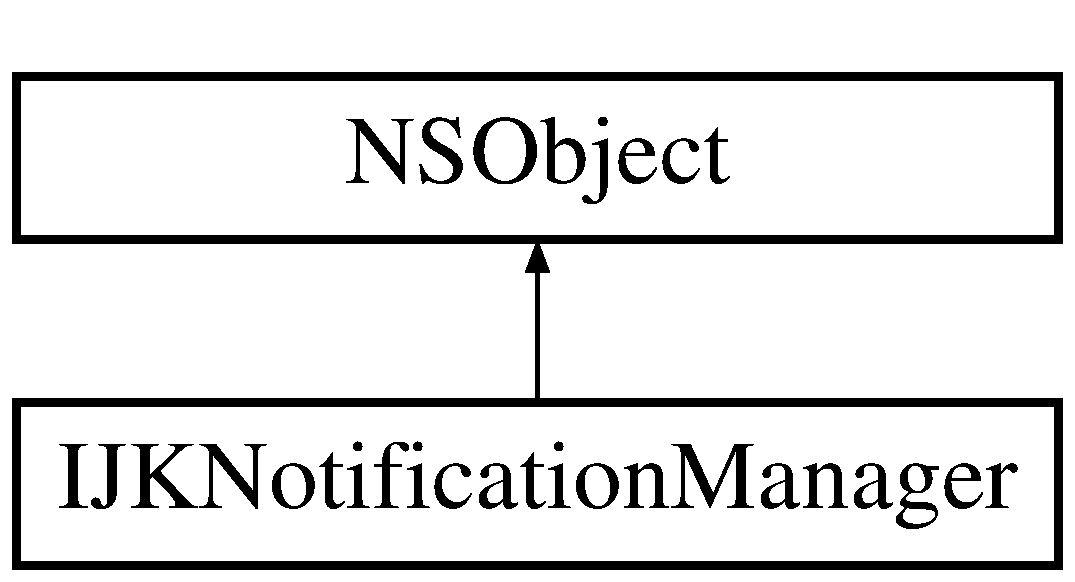
\includegraphics[height=2.000000cm]{interface_i_j_k_notification_manager}
\end{center}
\end{figure}
\subsection*{Instance Methods}
\begin{DoxyCompactItemize}
\item 
\mbox{\Hypertarget{interface_i_j_k_notification_manager_a1caa6c8b26b60d30fae4fd75047038ab}\label{interface_i_j_k_notification_manager_a1caa6c8b26b60d30fae4fd75047038ab}} 
(nullable instancetype) -\/ {\bfseries init}
\item 
\mbox{\Hypertarget{interface_i_j_k_notification_manager_a72c45d5667f3200d7a8bdced9cda19aa}\label{interface_i_j_k_notification_manager_a72c45d5667f3200d7a8bdced9cda19aa}} 
(void) -\/ {\bfseries add\+Observer\+:selector\+:name\+:object\+:}
\item 
\mbox{\Hypertarget{interface_i_j_k_notification_manager_a892a0796787e0fd89030aa97c75f6b96}\label{interface_i_j_k_notification_manager_a892a0796787e0fd89030aa97c75f6b96}} 
(void) -\/ {\bfseries remove\+All\+Observers\+:}
\end{DoxyCompactItemize}


The documentation for this class was generated from the following file\+:\begin{DoxyCompactItemize}
\item 
I\+J\+K\+Notification\+Manager.\+h\end{DoxyCompactItemize}

%--- End generated contents ---

% Index
\backmatter
\newpage
\phantomsection
\clearemptydoublepage
\addcontentsline{toc}{chapter}{Index}
\printindex

\end{document}
